\subsection{Построение математической модели}

Рассмотрим ``перевёрнутый'' маятник, схематично изображённый на Рис.~\ref{img:balance_picture}.
Будем считать, что вся масса маятника сосредоточенна в одной точке~--- точке маятника, максимально удалённой от шарнира.
Кроме того считаем, что сила сопротивления спиралевидной пружины приложена к той же точке.

\begin{figure}[h]
	\centering
	\begin{minipage}{0.45\linewidth}
		\centering
		\tikzset{every picture/.style={line width=0.75pt}} %set default line width to 0.75pt        

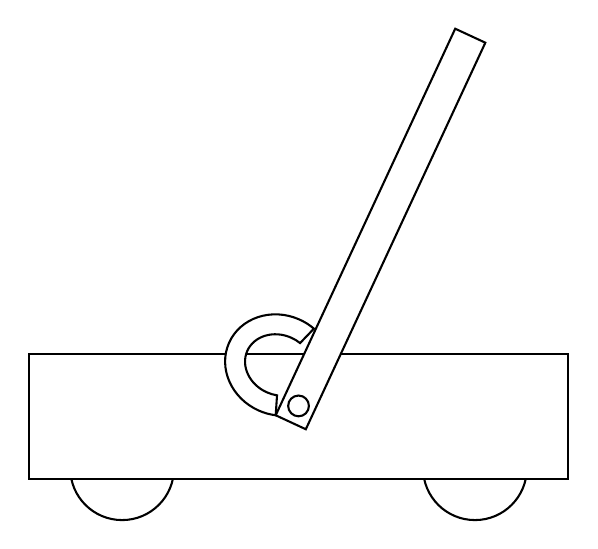
\begin{tikzpicture}[x=0.75pt,y=0.75pt,yscale=-1,xscale=1]
%uncomment if require: \path (0,300); %set diagram left start at 0, and has height of 300

%Shape: Circle [id:dp3063557070520314] 
\draw   (50,235) .. controls (50,221.19) and (61.19,210) .. (75,210) .. controls (88.81,210) and (100,221.19) .. (100,235) .. controls (100,248.81) and (88.81,260) .. (75,260) .. controls (61.19,260) and (50,248.81) .. (50,235) -- cycle ;
%Shape: Circle [id:dp031158162374192] 
\draw   (220,235) .. controls (220,221.19) and (231.19,210) .. (245,210) .. controls (258.81,210) and (270,221.19) .. (270,235) .. controls (270,248.81) and (258.81,260) .. (245,260) .. controls (231.19,260) and (220,248.81) .. (220,235) -- cycle ;
%Shape: Rectangle [id:dp857448713383056] 
\draw  [fill={rgb, 255:red, 255; green, 255; blue, 255 }  ,fill opacity=1 ] (30,180) -- (290,180) -- (290,240) -- (30,240) -- cycle ;
%Flowchart: Process [id:dp21554673154324455] 
\draw  [fill={rgb, 255:red, 255; green, 255; blue, 255 }  ,fill opacity=1 ] (149,209.5) -- (235.49,23.26) -- (250,30) -- (163.51,216.24) -- cycle ;
%Shape: Circle [id:dp9739998479490485] 
\draw   (155,205) .. controls (155,202.24) and (157.24,200) .. (160,200) .. controls (162.76,200) and (165,202.24) .. (165,205) .. controls (165,207.76) and (162.76,210) .. (160,210) .. controls (157.24,210) and (155,207.76) .. (155,205) -- cycle ;
%Shape: Block Arc [id:dp36869036397966315] 
\draw  [fill={rgb, 255:red, 255; green, 255; blue, 255 }  ,fill opacity=1 ] (149,209.5) .. controls (146.29,209.17) and (143.57,208.43) .. (140.91,207.26) .. controls (127.6,201.39) and (121.15,186.79) .. (126.5,174.65) .. controls (131.86,162.51) and (146.99,157.44) .. (160.3,163.31) .. controls (162.96,164.48) and (165.34,165.99) .. (167.41,167.77) -- (160.74,174.72) .. controls (159.47,173.69) and (158.02,172.8) .. (156.42,172.1) .. controls (147.97,168.37) and (138.51,171.25) .. (135.29,178.53) .. controls (132.08,185.81) and (136.33,194.74) .. (144.79,198.47) .. controls (146.39,199.18) and (148.02,199.64) .. (149.64,199.89) -- cycle ;




\end{tikzpicture}
	\end{minipage}
	\begin{minipage}{0.45\linewidth}
		\centering
		

\tikzset{every picture/.style={line width=0.75pt}} %set default line width to 0.75pt        

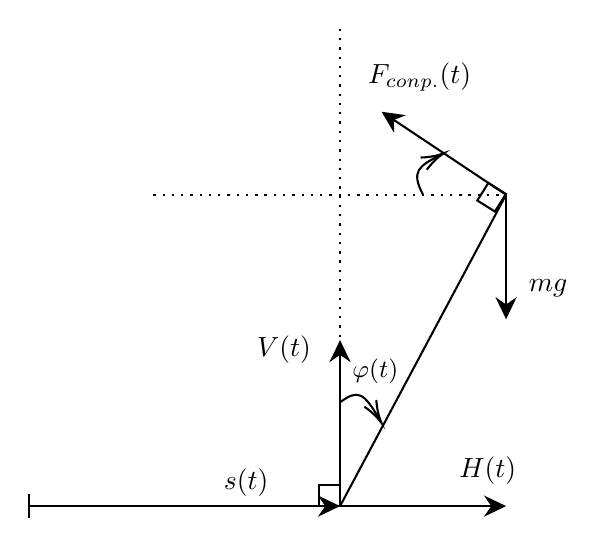
\begin{tikzpicture}[x=0.75pt,y=0.75pt,yscale=-1,xscale=1]
%uncomment if require: \path (0,300); %set diagram left start at 0, and has height of 300

%Straight Lines [id:da9082960361623723] 
\draw    (40,250) -- (187,250) ;
\draw [shift={(190,250)}, rotate = 180] [fill={rgb, 255:red, 0; green, 0; blue, 0 }  ][line width=0.08]  [draw opacity=0] (10.72,-5.15) -- (0,0) -- (10.72,5.15) -- (7.12,0) -- cycle    ;
\draw [shift={(40,250)}, rotate = 180] [color={rgb, 255:red, 0; green, 0; blue, 0 }  ][line width=0.75]    (0,5.59) -- (0,-5.59)   ;
%Straight Lines [id:da619700854654778] 
\draw    (270,100) -- (190,250) ;
%Straight Lines [id:da2680213245501296] 
\draw    (270,100) -- (270,157) ;
\draw [shift={(270,160)}, rotate = 270] [fill={rgb, 255:red, 0; green, 0; blue, 0 }  ][line width=0.08]  [draw opacity=0] (10.72,-5.15) -- (0,0) -- (10.72,5.15) -- (7.12,0) -- cycle    ;
%Straight Lines [id:da8310917143221241] 
\draw    (270,100) -- (212.5,61.66) ;
\draw [shift={(210,60)}, rotate = 393.69] [fill={rgb, 255:red, 0; green, 0; blue, 0 }  ][line width=0.08]  [draw opacity=0] (10.72,-5.15) -- (0,0) -- (10.72,5.15) -- (7.12,0) -- cycle    ;
%Straight Lines [id:da8347318970212223] 
\draw    (190,250) -- (267,250) ;
\draw [shift={(270,250)}, rotate = 180] [fill={rgb, 255:red, 0; green, 0; blue, 0 }  ][line width=0.08]  [draw opacity=0] (10.72,-5.15) -- (0,0) -- (10.72,5.15) -- (7.12,0) -- cycle    ;
%Straight Lines [id:da0962341838743137] 
\draw    (190,250) -- (190,173) ;
\draw [shift={(190,170)}, rotate = 450] [fill={rgb, 255:red, 0; green, 0; blue, 0 }  ][line width=0.08]  [draw opacity=0] (10.72,-5.15) -- (0,0) -- (10.72,5.15) -- (7.12,0) -- cycle    ;
%Straight Lines [id:da41784265135185517] 
\draw  [dash pattern={on 0.84pt off 2.51pt}]  (190,20) -- (190,250) ;
%Curve Lines [id:da2623450692945557] 
\draw    (190,200) .. controls (198.64,193.6) and (201.44,195.19) .. (209.03,208.3) ;
\draw [shift={(210,210)}, rotate = 240.4] [color={rgb, 255:red, 0; green, 0; blue, 0 }  ][line width=0.75]    (10.93,-3.29) .. controls (6.95,-1.4) and (3.31,-0.3) .. (0,0) .. controls (3.31,0.3) and (6.95,1.4) .. (10.93,3.29)   ;
%Straight Lines [id:da07376152116457713] 
\draw  [dash pattern={on 0.84pt off 2.51pt}]  (100,100) -- (270,100) ;
%Curve Lines [id:da8812105788162867] 
\draw    (230,100) .. controls (223.98,88.6) and (227.89,86.23) .. (238.3,80.87) ;
\draw [shift={(240,80)}, rotate = 512.78] [color={rgb, 255:red, 0; green, 0; blue, 0 }  ][line width=0.75]    (10.93,-3.29) .. controls (6.95,-1.4) and (3.31,-0.3) .. (0,0) .. controls (3.31,0.3) and (6.95,1.4) .. (10.93,3.29)   ;
%Shape: Rectangle [id:dp47533838253981786] 
\draw   (180,240) -- (190,240) -- (190,250) -- (180,250) -- cycle ;
%Shape: Rectangle [id:dp26114282721727233] 
\draw   (256.14,102.77) -- (261.45,94.3) -- (269.92,99.61) -- (264.61,108.08) -- cycle ;

% Text Node
\draw (148.75,238.63) node   [align=left] {\begin{minipage}[lt]{22.1pt}\setlength\topsep{0pt}
$\displaystyle s(t)$
\end{minipage}};
% Text Node
\draw (246,224.5) node [anchor=north west][inner sep=0.75pt]   [align=left] {$\displaystyle H(t)$};
% Text Node
\draw (148.5,166.5) node [anchor=north west][inner sep=0.75pt]   [align=left] {$\displaystyle V(t)$};
% Text Node
\draw (202,35) node [anchor=north west][inner sep=0.75pt]   [align=left] {$\displaystyle F_{conp.}(t)$};
% Text Node
\draw (279.5,139.5) node [anchor=north west][inner sep=0.75pt]   [align=left] {$\displaystyle mg$};
% Text Node
\draw (194.5,177.5) node [anchor=north west][inner sep=0.75pt]  [font=\small] [align=left] {$\displaystyle \varphi ( t)$};


\end{tikzpicture}
	\end{minipage}
	\caption{Схематичное изображение маятника и сил, приложенных к нему.}
	\label{img:balance_picture}
\end{figure}

Пусть в момент времени~$t$ перемещение шарнира характеризуется функцией $s(t)$, а угловое отклонение маятника~--- функцией~$\varphi(t)$.
Обозначим за $H(t)$ и $V(t)$ соответственно горизонтальную и вертикальную силы реакции, приложенные к шарниру, а за $J$~--- момент инерции маятника относительно оси, проведённой через груз (так как вся масса маятника содержится в грузе, то $J = 0$).
Остальные использованные параметры описаны в предыдущем разделе.
Тогда для рассматриваемой системы справедливы следующие уравнения:
\begin{equation} \label{eq:modeling_1}
	\begin{aligned}
& m \frac{d^2}{dt^2}(s(t) + l \sin\varphi(t)) = H(t) - \xi\varphi(t)\cos\varphi(t);
\\
& m \frac{d^2}{dt^2}(l \cos\varphi(t)) = V(t) + \xi\varphi(t)\sin\varphi(t) - mg;
\\
& J \frac{d^2}{dt^2}\varphi(t) = lV(t)\sin\varphi(t) - lH(t)\cos\varphi(t) = 0;
\\
& M\frac{d^2}{dt^2}s(t) = u(t) - H(t) - k\frac{d}{dt}s(t).
	\end{aligned}
\end{equation}

С целью упрощения уравнений предположим, что масса груза $m$ много меньше массы тележки $M$, и поэтому пренебрежем горизонтальной реакцией $H(t)$ на движение тележки.
В итоге после преобразований уравнений \eqref{eq:modeling_1} получим:
\begin{equation*}
	\begin{aligned}
&m \ddot s(t) + ml\ddot\varphi(t)\cos\varphi(t) - ml\varphi^2(t)\sin\varphi(t) = H(t) - \xi\varphi(t)\cos\varphi(t);
\\
&-ml\ddot\varphi(t)\sin\varphi(t) - ml\dot\varphi^2(t)\cos\varphi(t) = V(t) - mg + \xi\varphi(t)\sin\varphi(t);
\\
&V(t) = \frac{\cos\varphi(t)}{\sin\varphi(t)}H(t);
\\
&M\ddot s(t) = u(t) - k\dot s(t).
	\end{aligned}
\end{equation*}

Исключив из последних соотношений $H(t)$ и $V(t)$ получим окончательный закон движения рассматриваемой системы тел:
\begin{equation}\label{eq:modeling_equation}
	\begin{aligned}
&\ddot\varphi + \frac{\xi}{ml}\varphi - \frac{g}{l}\sin\varphi + \frac{1}{l}\ddot s \cos \varphi = 0;
\\
&M\ddot s = u - k\dot s.
	\end{aligned}
\end{equation}
Таким образом, введя вектор $x = [\varphi,\,\dot\varphi,\,s,\,\dot s]\T$, получим нелинеаризованную систему:
\begin{equation}\label{eq:modeling_system}
	\left\{
	\begin{aligned}
\dot x_1 &= x_2
\\
\dot x_2 &= -\frac{\xi}{ml}x_1 + \frac{g}{l}\sin x_1 - \frac{1}{Ml}(u - kx_4)\cos x_1
\\
\dot x_3 &= x_4
\\
\dot x_4 &= \frac{u}{M} - \frac{k}{M}x_4.
	\end{aligned}
	\right.
\end{equation}
